\documentclass[pdflatex,compress,mathserif]{beamer}

%\usetheme[dark,framenumber,totalframenumber]{ElektroITK}
\usetheme[darktitle,framenumber,totalframenumber]{ElektroITK}

\usepackage[utf8]{inputenc}
\usepackage[T1]{fontenc}
\usepackage{lmodern}
\usepackage[bahasai]{babel}
\usepackage{amsmath}
\usepackage{amsfonts}
\usepackage{amssymb}
\usepackage{graphicx}
\usepackage{multicol}
\usepackage{lipsum}
\usepackage{media9}
\usefonttheme[onlymath]{serif}

\newcommand*{\Scale}[2][4]{\scalebox{#1}{$#2$}}%

\renewcommand\thempfootnote{\arabic{mpfootnote}} % footnote arabic number

\setbeamertemplate{caption}[numbered]

\title{KECERDASAN BUATAN}
\subtitle{PARTICLE SWARM OPTIMIZATION (PSO)}

\author{Mifta Nur Farid}
\date{8 Februari 2024}

\begin{document}

\maketitle

\begin{frame}{What is Particle Swarm Optimization}
	\begin{definition}
		\stepcounter{footnote}
		Particle swarm optimization is a \textbf{stochastic population} based \textbf{optimization approach}, first published by Kennedy and Eberhart in 1995\footnote{Kennedy, J. and Eberhart, R. (1995) Particle Swarm Optimization. Proceedings of the IEEE International Conference on Neural Networks, 4, 1942-1948.}
	\end{definition}
\end{frame}

\begin{frame}{Optimization}
	\begin{itemize}
		\item \textbf{Optimization problem:} Maximizing or minimizing some function relative to some set, often representing a range of choices available in a certain situation
		\item Ex: Minimize $f(x,y) = (x^2 + y - 11)^2 + (x+y^2-7)^2$
		\centering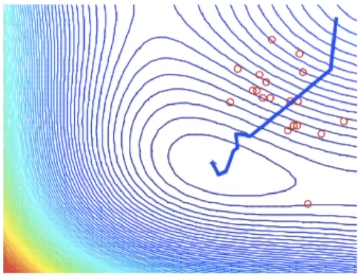
\includegraphics[width=0.6\linewidth]{img/01}
	\end{itemize}
\end{frame}

\begin{frame}{Optimization}
	\begin{itemize}
		\item Common applications of optimization:
		\begin{enumerate}
			\item Minimal cost
			\item Maximal profit
			\item Minimal error
			\item Optimal design
			\item Optimal management
			\item Variational principles
		\end{enumerate}
	\end{itemize}
\end{frame}

\begin{frame}{Introduction on PSO}
	\begin{itemize}
		\item Inspired by social behavior of birds and fishes
		\item Combines self-experience with social experience
		\item Population-based optimization
	\end{itemize}
	\begin{multicols}{2}
		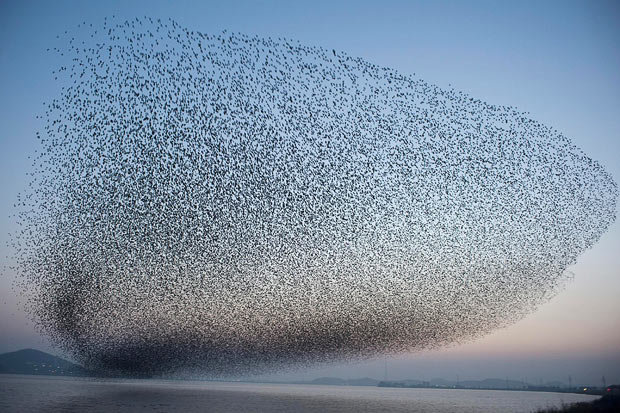
\includegraphics[width=\linewidth]{img/02}
		\columnbreak
		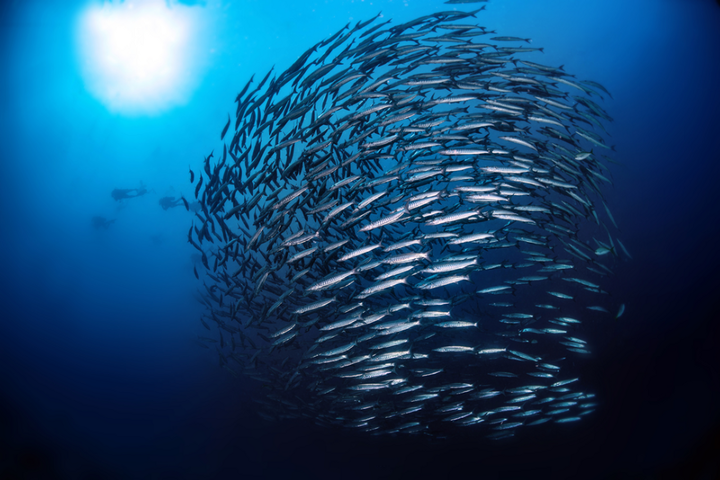
\includegraphics[width=\linewidth]{img/03}
	\end{multicols}
	\centering \href{https://www.youtube.com/watch?v=V4f\_1\_r80RY}{https://www.youtube.com/watch?v=V4f\_1\_r80RY}
\end{frame}

\begin{frame}{Introduction to the PSO: Origins}
	\begin{itemize}
		\item In 1986, Craig Reynolds described this process in 3 simple behaviors:
	\end{itemize}
	\begin{multicols}{3}
		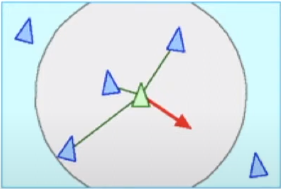
\includegraphics[width=\linewidth]{img/04}
		\scriptsize{\textbf{Separations}:\\
			avoid crowding local flockmates}
		\vfill\null
		\columnbreak
		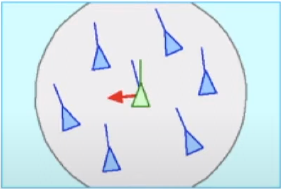
\includegraphics[width=\linewidth]{img/05}
		\scriptsize{\textbf{Alignments}:\\
			move towards the average heading of local flockmates}
		\vfill\null
		\columnbreak
		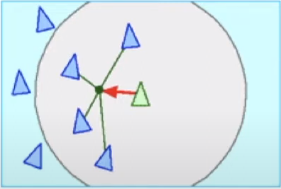
\includegraphics[width=\linewidth]{img/06}
		\scriptsize{\textbf{Cohesion}:\\
			move toward the average position of local flockmates}
		\vfill\null
	\end{multicols}
	\centering \href{https://www.youtube.com/watch?v=gkGa6WZpcQg}{\footnotesize{https://www.youtube.com/watch?v=gkGa6WZpcQg}}
\end{frame}

\begin{frame}{Origins and Inspiration from Natural Systems}
	Developed by \textbf{Jim Kennedy}, Bureau of Labor Statistics, U.S. Department of Labor and \textbf{Russ Ebenhart}, Computer Science, Purdue University at 1995.
\end{frame}

\begin{frame}
	\Large{So with the inspiration from nature, how do you think the idea can be adopted for solving optimization problem?}
\end{frame}

\begin{frame}{Scenario}
	\begin{itemize}
		\item As stated before, PSO simulates the behaviors of bird flocking.
		\item Suppose the following scenario:
	\end{itemize}
	\begin{exampleblock}{Scenario:}
		A group of birds are randomly searching food in an area. There is only one piece of food in the area being searched. All the birds do not know where the food is. But they know how far the food is in each iteration. So what is the best strategy to find the food?\footnote{http://www.swarmintelligence.org/tutorials.php}
	\end{exampleblock}
\end{frame}

\begin{frame}{Scenario}
	\begin{exampleblock}{Scenario:}
		A group of birds are randomly searching food in an area. There is only one piece of food in the area being searched. All the birds do not know where the food is. But they know how far the food is in each iteration. So what is the best strategy to find the food?\footnote{http://www.swarmintelligence.org/tutorials.php}
	\end{exampleblock}
	\begin{alertblock}{The best strategy:}
		The effective one is to follow the bird which is nearest to the food.
	\end{alertblock}
\end{frame}

\begin{frame}{Concept}
	\begin{itemize}
		\item Uses a number of particles that constitute a swarm moving around in the search space looking for the best solution.
		\item Each particle in the search space adjusts its "flying" according to its \emph{own flying experience} as well as the \emph{flying experience of other particles}.
	\end{itemize}
	\begin{multicols}{2}
		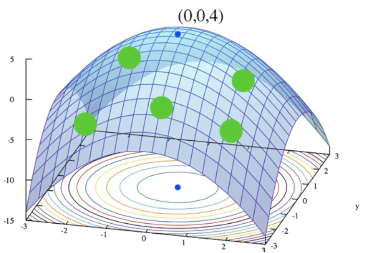
\includegraphics[width=\linewidth]{img/07}
		\columnbreak
		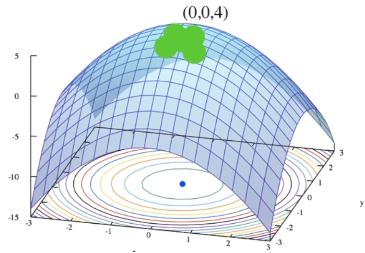
\includegraphics[width=\linewidth]{img/08}
	\end{multicols}
\end{frame}

\begin{frame}{Particle Swarm Optimization}
	\begin{itemize}
		\item Swarm: a set of particles ($S$)
		\item Particle: a potential solution
		\begin{itemize}
			\item Position: $X_i = (x_{i1},x_{i2},\dots,x_{in}) \in \mathbb{R}^n$
			\item Velocity: $V_i = (v_{i1},v_{i2},\dots,v_{in}) \in \mathbb{R}^n$
		\end{itemize}
		\item Each particle maintains individual best position:
		\item[] $P_i = (p_{i1}, p_{i2}, \dots, p_{in}) \in \mathbb{R}^n$
		\item[] $\text{PBest}_i = f(P_i)$
		\item Swarm maintains its global best:
		\item[] $P_g \in \mathbb{R}^n$
		\item[] $\text{GBest} = f(P_g)$
	\end{itemize}
\end{frame}

\begin{frame}{PSO Algorithm}
	\begin{itemize}
		\item Original velocity update equation
		\begin{align*}
			\mathbf{v}_i (k+1) =&~ \text{inertia} + \text{cognitive} + \text{social} \\
			\mathbf{v}_i(k+1) =&~ \omega \mathbf{v}_i(k) + c_1 \text{random}_1()(\text{PBest}_i - \mathbf{x}_i(k))\\
			&+ c_2 \text{random}_2()(\text{GBest} - \mathbf{x}_i(k))
		\end{align*}
		\begin{itemize}
			\item $\omega$, $c_1$, $c_2$: constant
			\item $\text{random}_1()$, $\text{random}_2()$: random variable
		\end{itemize}
		\item Position update: $\mathbf{x}_i(k+1) = \mathbf{x}_i(k) + \mathbf{v}_i(k+1)$
	\end{itemize}
\end{frame}

\begin{frame}{PSO Algorithm}
	Basic algorithm of PSO
	\begin{enumerate}
		\item Initialize the swarm form the solution space 
		\item Evaluate the fitness of each particle \label{step2}
		\item Update individual and global best
		\item Update velocity and position of each particle
		\item Go to step \ref{step2}, and repeat until termination condition
	\end{enumerate}
\end{frame}

\begin{frame}{PSO Algorithm}
	Particle's velocity: $$\mathbf{v}_i (k+1) = \text{inertia} + \text{cognitive} + \text{social}$$
	\begin{figure}
		\centering
		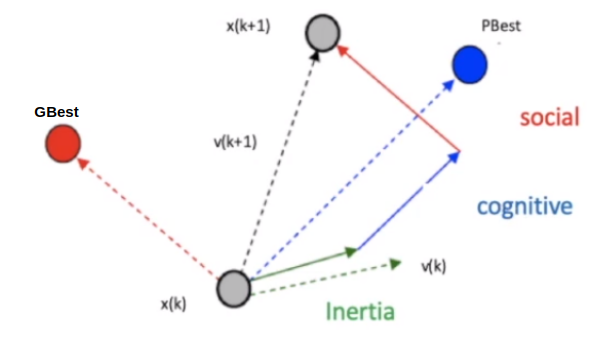
\includegraphics[width=0.7\linewidth]{img/09}
	\end{figure}
\end{frame}

\begin{frame}{PSO solution update in 2D}
	\begin{multicols}{2}
		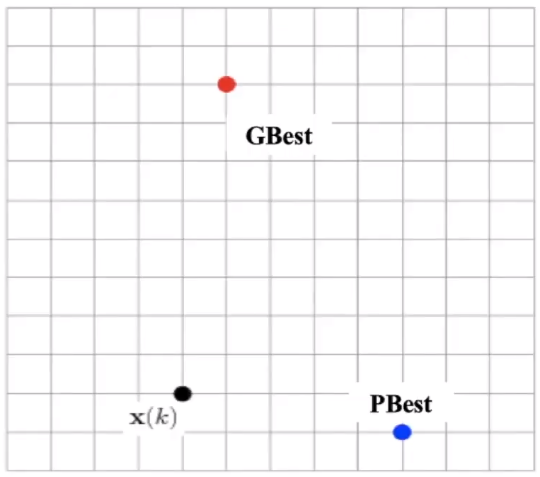
\includegraphics[width=\linewidth]{img/10}
		\vfill\null
		\columnbreak
		\begin{itemize}
			\item[] \scriptsize{$\mathbf{x}(k)$: current solution $(4,2)$}
			\item[] \scriptsize{$\text{PBest}$: particle's best solution $(9,1)$}
			\item[] \scriptsize{$\text{GBest}$: global best solution $(5,10)$}
		\end{itemize}
		\vfill\null
	\end{multicols}
\end{frame}

\begin{frame}{PSO solution update in 2D}
	\begin{multicols}{2}
		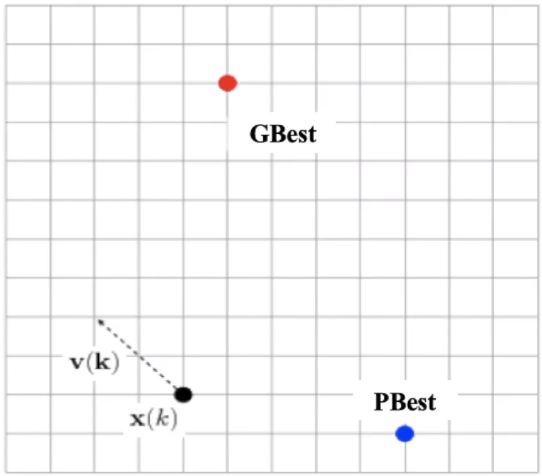
\includegraphics[width=\linewidth]{img/11}
		\vfill\null
		\columnbreak
		\begin{itemize}
			\item[] \scriptsize{$\mathbf{x}(k)$: current solution $(4,2)$}
			\item[] \scriptsize{$\text{PBest}$: particle's best solution $(9,1)$}
			\item[] \scriptsize{$\text{GBest}$: global best solution $(5,10)$}
			\item[] 
			\item[] \scriptsize{$\text{Inertia}$: $\mathbf{v}(k) = (-2,2)$}
		\end{itemize}
		\vfill\null
	\end{multicols}
\end{frame}

\begin{frame}{PSO solution update in 2D}
	\begin{multicols}{2}
		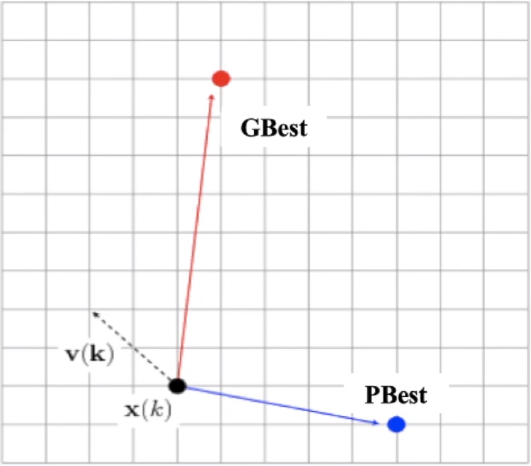
\includegraphics[width=\linewidth]{img/12}
		\vfill\null
		\columnbreak
		\begin{itemize}
			\item[] \scriptsize{$\mathbf{x}(k):$ current solution $(4,2)$}
			\item[] \scriptsize{$\text{PBest}:$ particle's best solution $(9,1)$}
			\item[] \scriptsize{$\text{GBest}:$ global best solution $(5,10)$}
			\item[]
			\item[] \scriptsize{$\text{Inertia}$: $\mathbf{v}(k) = (-2,2)$}
			\item[] \scriptsize{$\text{Cognitive}$:\\
				$\text{PBest} - \mathbf{x}(k) = (9,1) - (4,2) = (5,-1)$}
			\item[] \scriptsize{$\text{Social}$:\\
				$\text{GBest} - \mathbf{x}(k) = (5,10) - (4,2) = (1,8)$}
		\end{itemize}
		\vfill\null
	\end{multicols}
\end{frame}

\begin{frame}{PSO solution update in 2D}
	\begin{multicols}{2}
		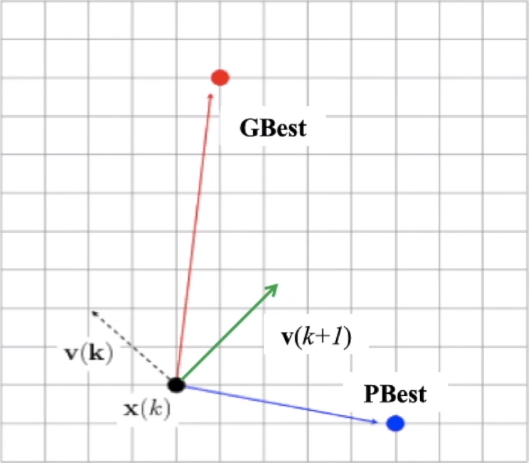
\includegraphics[width=\linewidth]{img/13}
		\vfill\null
		\columnbreak
		\begin{itemize}
			\item[] \scriptsize{$\mathbf{x}(k):$ current solution $(4,2)$}
			\item[] \scriptsize{$\text{PBest}:$ particle's best solution $(9,1)$}
			\item[] \scriptsize{$\text{GBest}:$ global best solution $(5,10)$}
			\item[]
			\item[] \scriptsize{$\text{Inertia}$: $\mathbf{v}(k) = (-2,2)$}
			\item[] \scriptsize{$\text{Cognitive}$:\\
				$\text{PBest} - \mathbf{x}(k) = (9,1) - (4,2) = (5,-1)$}
			\item[] \scriptsize{$\text{Social}$:\\
				$\text{GBest} - \mathbf{x}(k) = (5,10) - (4,2) = (1,8)$}
			\item[]
			\item[] $\mathbf{v}(k+1) = (-2,2) + 0.8(5,-1) + 0.2(1,8) = (2.2,2.8)$
		\end{itemize}
		\vfill\null
	\end{multicols}
\end{frame}

\begin{frame}{PSO solution update in 2D}
	\begin{multicols}{2}
		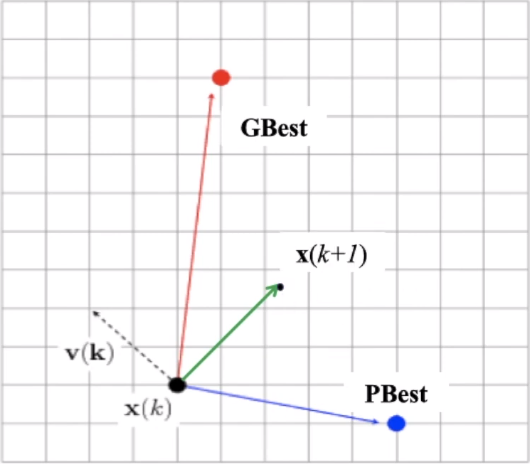
\includegraphics[width=\linewidth]{img/14}
		\columnbreak
		\begin{itemize}
			\item[] \scriptsize{$\mathbf{x}(k):$ current solution $(4,2)$}
			\item[] \scriptsize{$\text{PBest}:$ particle's best solution $(9,1)$}
			\item[] \scriptsize{$\text{GBest}:$ global best solution $(5,10)$}
			\item[]
			\item[] \scriptsize{$\text{Inertia}$: $\mathbf{v}(k) = (-2,2)$}
			\item[] \scriptsize{$\text{Cognitive}$:\\
				$\text{PBest} - \mathbf{x}(k) = (9,1) - (4,2) = (5,-1)$}
			\item[] \scriptsize{$\text{Social}$:\\
				$\text{GBest} - \mathbf{x}(k) = (5,10) - (4,2) = (1,8)$}
			\item[]
			\item[] $\mathbf{v}(k+1) = (-2,2) + 0.8(5,-1) + 0.2(1,8) = (2.2,2.8)$
			\item[] $\mathbf{x}(k+1) = \mathbf{x}(k) + \mathbf{v}(k+1) = (4,2) + (2.2,2.8) = (6.2, 4.8)$
		\end{itemize}
		\vfill\null
	\end{multicols}
\end{frame}

\begin{frame}{Example}
	Find the minimum of this function
	$$f(x) = 3x_1^2 - 2x_1x_2 + 3x_2^2 - x_1 - x_2$$
	\begin{figure}
		\centering
		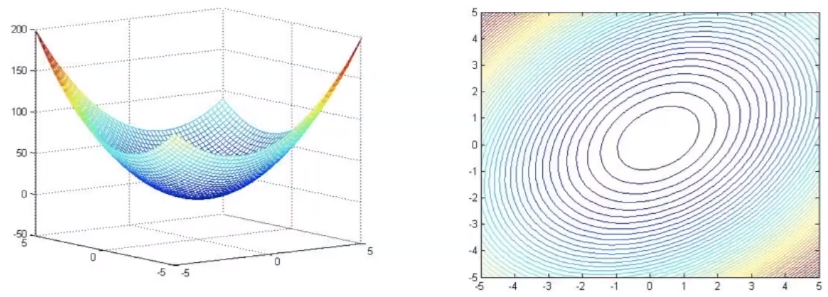
\includegraphics[width=\linewidth]{img/15}
	\end{figure}
\end{frame}

\begin{frame}{Example}
	\scriptsize$$f(x) = 3x_1^2 - 2x_1x_2 + 3x_2^2 - x_1 - x_2$$
	\begin{figure}
		\centering
		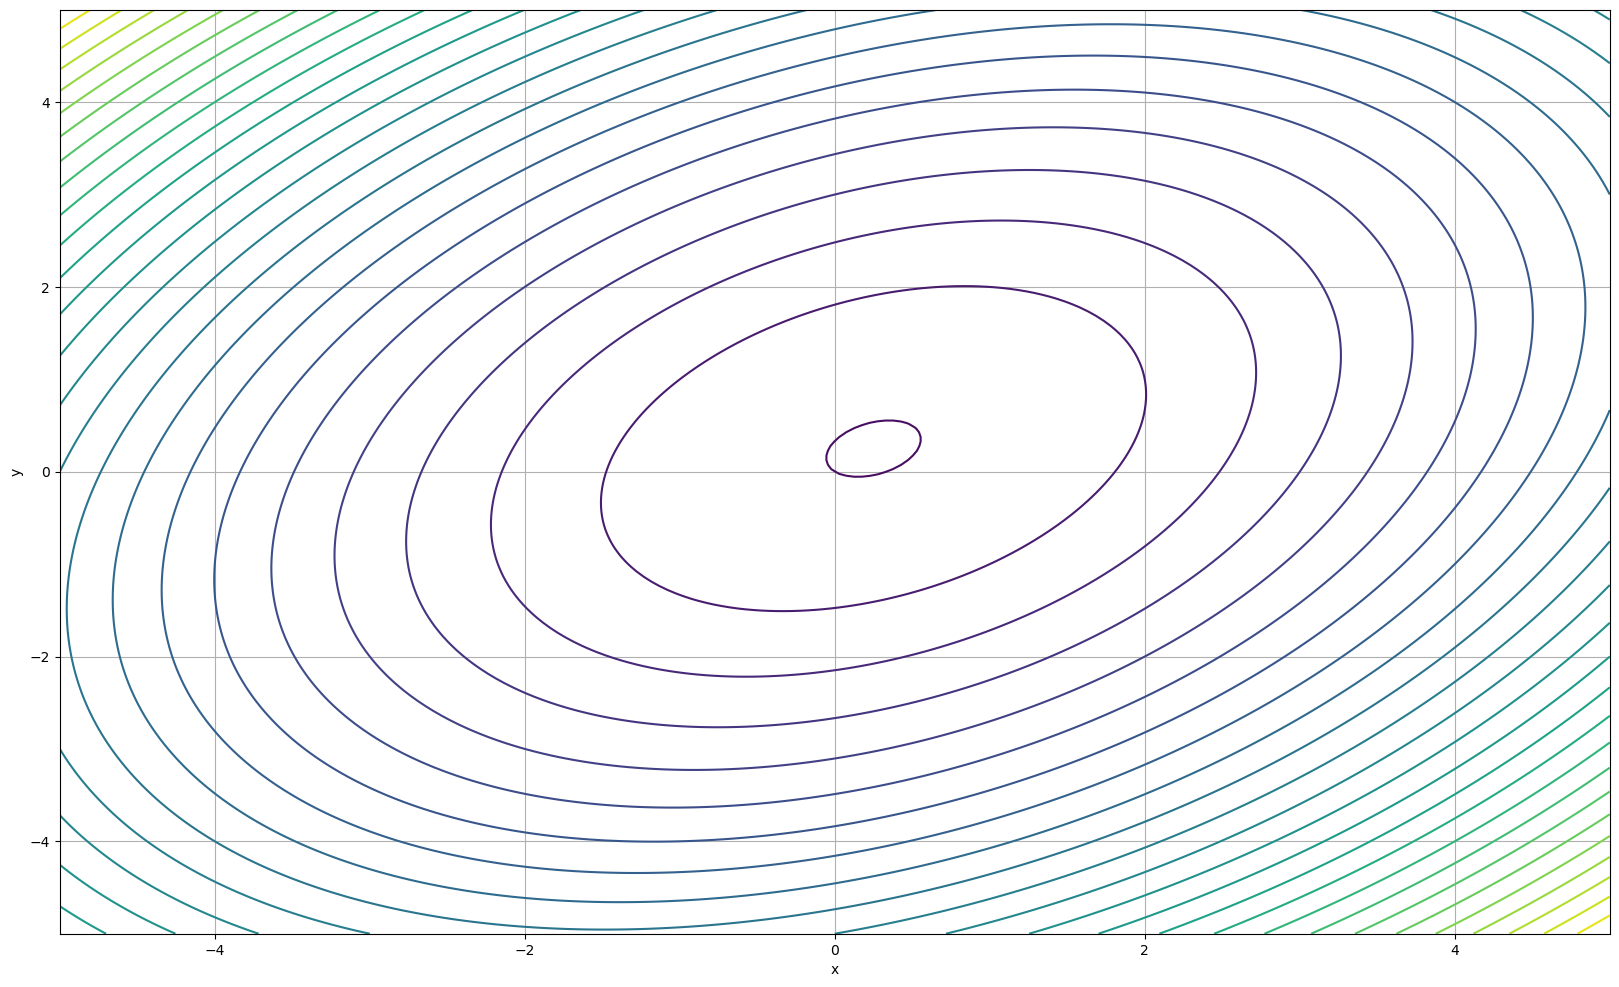
\includegraphics[width=0.8\linewidth]{img/15a}
	\end{figure}
\end{frame}

\begin{frame}{Example}
	\begin{figure}
		\centering
		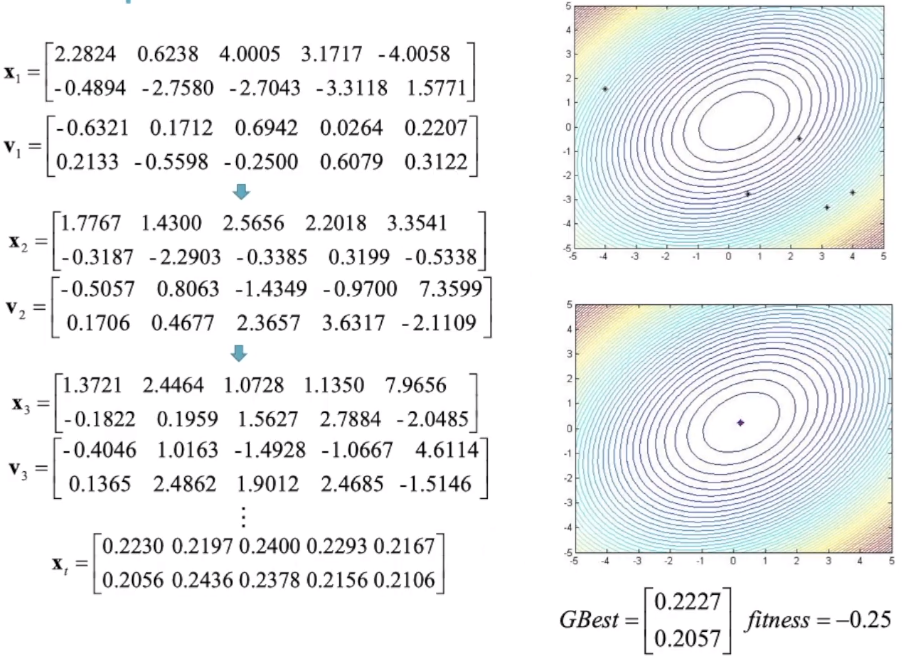
\includegraphics[width=\linewidth]{img/16}
	\end{figure}
\end{frame}

\begin{frame}
	\centering
	\LARGE{THANK YOU\\}
	\vspace{0.5cm}
	\large{\emph{Any Question?}}
\end{frame}

\end{document}
